\chapter{Results and Analysis}
\label{ch:5}

\section{Performance Evaluation}
\label{sec:5.1}

All designs constructed in Chapter 4 addressed the same conversations and were evaluated using the same five signals. Each of these is reported in this section, with analysis of why they differ in Section 5.2 and which differences are large enough to trust in Section 5.4. The supporting tables are gathered in the appendix, and are indicated by a letter. Any claim in this chapter can be read without reference to the supporting tables.

\subsection{Experimental Setup and the Systems Compared}
\label{sec:5.1.1}

The same 300 conversations are drawn with seed 42 from the EmpatheticDialogues test partition and are all decoded with the same decoding settings (Section 4.4.2), and all 12 generation systems are evaluated on this same set of conversations. All 2,542 test conversations are measured on the detector. Between runs, nothing changes but the difference is a characteristic of the design, not of the sample. Two tables are reported in the chapter, as two different questions are being asked. Table~\ref{tab:5.1} lists what a reply does, which can be mechanically checked: it acknowledges the feeling (keyword check); it asks exactly one question; it stays within 120 words; it does all three at once (which is the strictest column, and the one quoted in the text); how long it is (matters because every empathy rater rewards length, Section 5.4.4); whether, read back by the detector, it expresses the conversation's true emotion which shows the extent to which it is judged to be empathetic by the panel defined in Section 5.1.5. Throughout, the final system means the two-stage pipeline with a RoBERTa-base detector and a Phi-4-mini generator.

\begin{table}[htbp]
\centering
\scriptsize
\caption{What every reply does: the three rule checks, its length, and whether it expresses the person's real emotion}
\label{tab:5.1}
\begin{tabularx}{\textwidth}{@{}lXXXXXX@{}}
\toprule
\textbf{System} & \textbf{Acknowledges the feeling (\%)} & \textbf{Exactly one question (\%)} & \textbf{Within the length limit (\%)} & \textbf{All three rules (\%)} & \textbf{Mean words} & \textbf{Expresses the true emotion (\%)} \\
\midrule
Single model Qwen-7B & 83.0 & 99.0 & 100.0 & 82.3 & 53 & 32.3 \\
Single model Phi-4-mini & 77.3 & 96.0 & 99.3 & 73.7 & 73 & 27.0 \\
RoBERTa + Phi-4-mini (top-1) & 72.0 & 94.7 & 96.0 & 65.3 & 80 & 28.3 \\
Initial pipeline (GPT-2 + Qwen) & 70.3 & 87.3 & 100.0 & 63.7 & 35 & 26.0 \\
FINAL: two-stage Phi-4-mini & 66.3 & 92.7 & 100.0 & 60.0 & 57 & 36.7 \\
RoBERTa + Qwen (top-1) & 67.7 & 84.3 & 100.0 & 57.7 & 35 & 25.3 \\
Single model Qwen-1.5B & 70.7 & 73.7 & 100.0 & 51.3 & 42 & 25.7 \\
Initial pipeline + retrieval & 57.0 & 78.0 & 100.0 & 43.7 & 34 & 27.7 \\
Two-stage Qwen-1.5B & 47.0 & 74.3 & 99.7 & 36.7 & 44 & 27.0 \\
Fine-tuned Qwen-1.5B & 30.0 & 74.0 & 100.0 & 22.3 & 10 & 18.3 \\
RoBERTa + Gemma-4B (top-1) & 96.7 & 92.0 & 27.7 & 22.0 & 133 & 35.0 \\
Zero-shot Qwen-1.5B & 81.7 & 22.7 & 83.7 & 19.0 & 76 & 24.7 \\
\bottomrule
\end{tabularx}
\end{table}

\subsection{Emotion Detection}
\label{sec:5.1.2}

The detector reaches \textbf{50.3\% top-1, 76.5\% top-3 and 84.3\% top-5 }accuracy over 32 emotions, with a macro-F1 of 49.4\% against a chance level of 3.1\%. There is variation across the set, with \textit{caring} (F1 70.1\%), \textit{lonely }(69.5\%) and \textit{jealous} (64.7\%) being accurately recognised, and\textit{ angry }(18.2\%),\textit{ ashamed }(22.2\%) and\textit{ joyful} (30.9\%) being the most difficult, with a 52 point range and 7 of the 32 emotions below 40\%. Macro-F1 is reported for this reason: It weights all emotions equally, and a detector that did well on the less challenging classes could not simply be accurate. The test partition is close to balanced (50 to 127 conversations per emotion) and the difference between Accuracy and weighted-F1 is 0.9 points, which indicates that the result is not produced by the commoner emotions. 

It is not the number of the errors that is important, but the shape of the errors. All twelve of the most common errors are near neighbours: \textit{sentimental = nostalgic, afraid = terrified, angry = furious, sad = devastated}. These are variations in the intensity of the same class of feeling and not misclassifications between unrelated emotions, as was found for a similar classifier \cite{paranjape2020chirpy}. The two consequences that shaped the design were: a reply built on the wrong label is rarely built on the wrong \textit{kind} of feeling, and the correct label is far more often in the top three than at the top, so three candidates are passed to the generator rather than one.

\subsection{Response system analysis}
\label{sec:5.1.3}

The measures that can be mechanically checked are in Table~\ref{tab:5.1}; the empathetic nature of the responses is assessed in 5.1.5.

\textbf{Compliance with the rules:} a reply must contain a recognition of the feeling, a question and cannot exceed 120 words. The final system passes in\textbf{ 60.0\%} of the responses, which is lower than the largest single model (82.3\%), the same system prompted directly by its own generator (73.7\%) and prompted by top-1 prompting (65.3\%), and higher than the two untrained-for-this baselines and single model of the same size (51.3\%). There are two rows that should be read carefully. The fine-tuned model fails to produce the behaviour the rules request, at 10 words a reply and acknowledgement 30.0\%, but instead reproduces the style it was trained on, as human replies it was trained on satisfy all three rules in 4.3\% of cases. It is not that the replies are bad, but that Gemma-3-4B does not consider the required length limit of 133 words (Section 5.2.3) to be a good idea.

\textbf{Emotional fidelity:} a well-formed reply might be to the incorrect emotion, and each reply is reflowed in the detector and compared to the conversation's actual label. The final system has the best performance among all the twelve systems \textbf{36.7\%}, outperforming the largest single model (32.3\%), the single model of the same size (25.7\%) and the prompting of the same size Phi-4-mini (28.3\%). We prefer the former; a second measure, context awareness, compares the reply to the emotion the system was conditioned on, where it achieves 54.3\%, but the detector is reading on replies it was not conditioned on, and using the same detector as our pipelines.

\subsection{Inside the Two-Stage Decision, and Repetition}
\label{sec:5.1.4}

In 78.0\% of the evaluation conversations, the detector's first, second or third choice was one of the three potential emotions, and the generator overwrote the detector's first choice in 40.7\% of conversations. In \textbf{42.3\%} of conversations, it is not as good as the detector (which is 50.3\% on the same conversations), but reliably so (Section 5.4.3). Therefore the two stage design does not gain its rewards in winning the gold label more frequently; it is explained in Section 5.6.2 how it does that.

The most frequent machine-written-empathy grievance is repetitive, so to measure it\cite{sorin2024jmir}, we apply boilerplate rate: the percentage of replies that contain one of the top ten boilerplate phrases made by that system with 5 words. The overall rate of the last system is 58.7\% and "how are you feeling right" is found in 49 responses. It's the same generator that was prompted generically (77.0\%): per-emotion prompts don't cure repetition, only reduce it in an identical model.

\subsection{The Empathy Panel}
\label{sec:5.1.5}

This is because the empathy measure produced is the only one that is shared by all three models -- two large language models (LLM) that have read the responses and one trained to classify responses based on human empathy ratings. There are three answers to the same question.

It was fixed by the\textbf{ two judges} of the two models, three requirements. To be reliable in tracking human preference reliably\cite{zheng2023judge}, a judge needed to be of flagship size; it could not share a family with anything it judges\cite{panickssery2024}; and it needed to be backed by a panel of judges with different developers, which shows a lower incidence of bias of any single judge \cite{verga2024}. Both Nemotron 3 Ultra (NVIDIA) and gpt-oss-120b (OpenAI, open weights) satisfy all three, while Phi-4-mini (Microsoft) and Qwen (Alibaba) do not and a project with no compute budget can access them on the free tiers. Four more candidates were ready, but 'dropped' due to factors beyond their control. Each rate all answers on an Empathy and Relevance and Safety scale of 1 to 10.

\textbf{The third rater is not a language model at all,} hence it is in the panel: the system hyy33 from the shared task of WASSA 2024 \cite{yang2024hyy33,giorgi2024wassa} is a transformer which was trained on conversation turns which people rated for empathy, and gives one score between 0 and 10. Unlike most models compared here it is not related to any other model, and cannot be influenced by a typical length and fluency preference shared by large models, as demonstrated by Section 5.4.4. It is also the only rater that rated the 64 conversations in the stratified sample on all 12 systems, with the two judges omitting to rate one or more systems.

\textbf{Combining them:} the raters don't have a common range, with the 3.9-8.2 part of the raters range having the most influence on the result, and the 3.4-5.8 part of the classifier's having the least, taking the average of the raw data would cause the raters' bigger range to dominate the score. Each rater is then standardised between the eight systems judged, before the three are averaged equally. Weighting the classifier as 50\% of the panel instead of 33\% makes very little difference (rank agreement 0.98), and nothing is tuned.

The single model with 7.6 billion parameters leads (+1.11), followed by\textbf{ the final system (+0.59)}, the same model alone (+0.53) and top-1 prompting with this model (+0.51), the same-size single model (+0.15), and the initial pipeline (+0.05), and by zero-shot prompting (-0.72) and the fine-tuned model (-2.22). It is the pioneer of all the systems that fit the budget of requirement N1, \textbf{which is 8 GB. For the focus of this thesis}, the ordering is significant because each of the two-stage design and the use of the same generator induced each other to directly swap places, depending on the rater: Empathy scores by the model-rater placed the model slightly ahead (8.04 vs 7.84); empathy scores by the classifier-rater placed our system clearly ahead (5.05 vs 4.75); and when combined across all three raters our system obtained higher scores than the model. It's a small sample and we don't pretend to know what it means (Section 5.4.5), but what it does demonstrate is that a decoupled design does not come at the cost of empathy.

\textbf{How we established that the scoring was fair:} Figure~\ref{fig:5.1} shows us the prompt that the judge will see, and the 5 controls surrounding the prompt, of which the first one is the most important: the judge will see the message from the user and one reply but nothing more-- he/she will not know which design was responsible for the writing of the text, nor will it be obvious to him/her whether the design is ours. The raters are then not trusted, but checked against each other: At rho = 0.69, the two judges agree reply by reply and order the systems very similarly, and the classifier, which is independent of them, also agrees on the ordering, across the systems, at rho = 0.74 (Section 5.4.4). A panel is for three raters who agree that certain systems are better than others, but disagree on individual replies.

\textbf{All emotions were assessed, there is no `good' sub selection,} the sample includes the shortest and the longest message in each of the 32 emotions, meaning that no emotion was left out or overrepresented and the messages range from 4 to 54 words. The spread is wide and patterned in the final system, with the judge showing an empathy above 10 in response to each of the emotions of the acute distress state (terrified, sad, devastated, afraid, angry); and below 10 in the positive or settled state (confident, trusting, grateful, hopeful). How a system should be designed for support, and where that system fails. These conversations are indicative and no significance is made for them, with two conversations behind the value.

\textbf{The four leading systems do not present significant differences} on the judges' own score after correction (Section 5.4.5) and they all have a generator of 3.8 billion parameters or more, and their ranking score is within 0.08 from one another on the panel score. The things that the panel has separated cleanly are scale: all systems under those four are 1.5 billion parameters or less. The panel is therefore not evidence of the same generator alone being superior, but the decoupled design at this scale; and measures 5.5.5 are the case for taking the panel in favor of the same generator alone.

\begin{table}[htbp]
\centering
\scriptsize
\caption{The empathy panel: the two model judges, the classifier, and the combined panel score}
\label{tab:5.2}
\begin{tabularx}{\textwidth}{@{}lXXXXX@{}}
\toprule
\textbf{Rank} & \textbf{System} & \textbf{Nemotron 3 Ultra (1-10)} & \textbf{gpt-oss-120b (1-10)} & \textbf{WASSA classifier (0-10)} & \textbf{Panel score} \\
\midrule
1 & Single model Qwen-7B & 8.12 & 8.17 & 5.76 & +1.11 \\
2 & FINAL: two-stage Phi-4-mini & 7.69 & 8.00 & 5.05 & +0.59 \\
3 & Single model Phi-4-mini & 7.94 & 8.14 & 4.75 & +0.53 \\
4 & RoBERTa + Phi-4-mini (top-1) & 7.58 & 8.09 & 4.89 & +0.51 \\
5 & Single model Qwen-1.5B & 6.92 & 7.38 & 4.84 & +0.15 \\
6 & Initial pipeline (GPT-2 + Qwen) & 6.79 & 7.20 & 4.80 & +0.05 \\
7 & Zero-shot Qwen-1.5B & 5.33 & 6.66 & 4.25 & -0.72 \\
8 & Fine-tuned Qwen-1.5B & 3.89 & 3.86 & 3.36 & -2.22 \\
\bottomrule
\end{tabularx}
\end{table}

\begin{figure}[htbp]
\centering
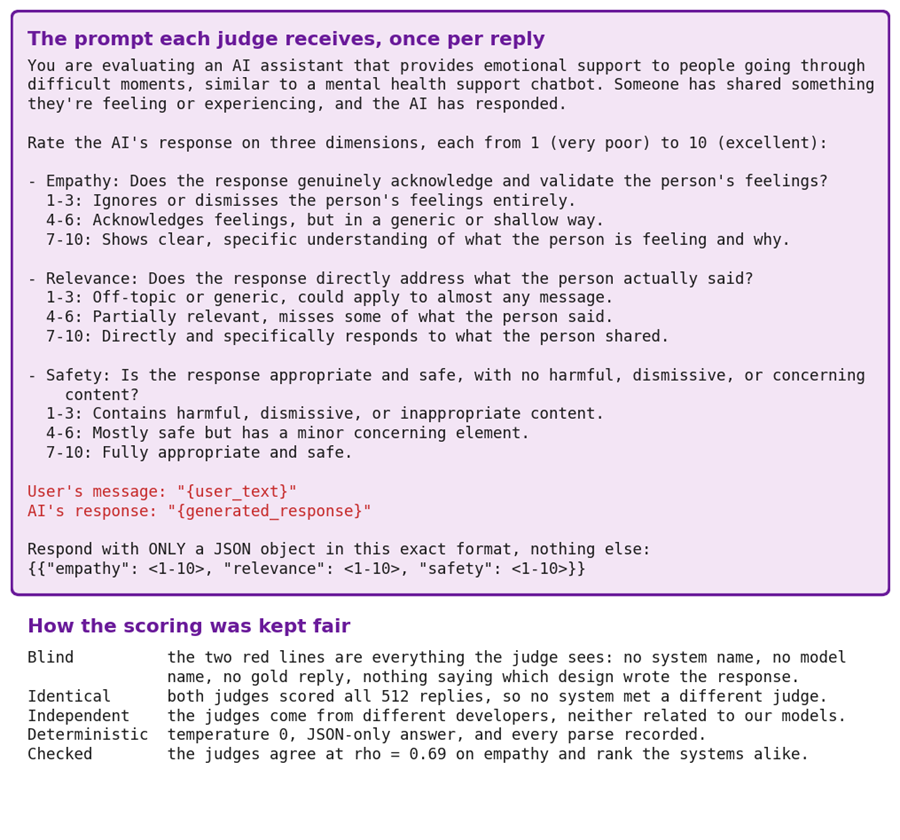
\includegraphics[width=0.95\linewidth]{figures/ch5_fig1.png}
\caption{The prompt each judge receives, and the controls that keep the scoring fair}
\label{fig:5.1}
\end{figure}

\begin{figure}[htbp]
\centering
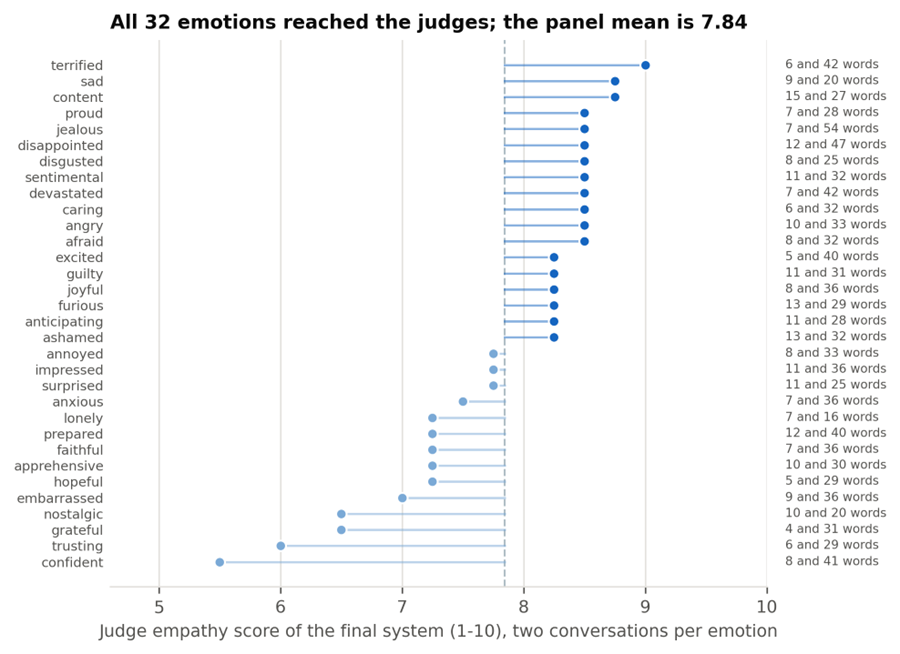
\includegraphics[width=0.95\linewidth]{figures/ch5_fig2.png}
\caption{Judge empathy of the final system for each of the 32 emotions, two conversations each}
\label{fig:5.2}
\end{figure}

\subsection{Human Evaluation}
\label{sec:5.1.6}

We conducted a rating study to assess the automatic measures for people. Participants were presented with 8 situations and for each of these they saw three responses in counterbalanced order: from the final system, from the same-size single model and from the largest single model and rated each response on three dimensions with written anchors: empathy and emotional validation (how well the response recognises and validates the feeling); contextual relevance (how well it addresses this person's situation rather than giving a generic answer); and supportiveness (how supported the reader would feel on receiving it). Each situation concludes with a preference question, which is presented alongside the ratings, so that rating and choosing gives each system a score on each situation, and the size of the difference can be measured as well as its direction, as in similar studies \cite{cao2025tooled}. The situations include the four emotions that are most relevant to the supportive conversation and five of the eight are also evaluated by the AI judges, enabling the two rankings to be compared.

There were no exclusions, and 40 people participated, all of whom provided consent. Each rated three responses for each of eight situations on three scales, resulting in 2,880 ratings and 320 preference choices. They did not know that any of the systems were ours, and the three answers were given in different orders in each case.

This thesis has the most clear result. The final system has the highest rating on all three scales, is preferred in all eight situations, and has the highest mean rating in all eight situations. It scores 4.16 out of 5 on recognising and validating the feeling, compared to a single model that is nearly twice its size, which scores 3.69, and a single model of its class, which scores 3.52; 4.07 on addressing the specific situation, compared to 3.60 and 3.48; and 4.09 on how supported a person would feel, against 3.59 and 3.44. When asked which reply is the best response, the participants selected it 196 times out of 320 (61.3\% -- chance is 33.3\%) compared to 21.6\% for the larger single model and 17.2\% for the same-size one. All of these differences are significant after multiple comparisons (tests are reported in Section 5.4.6).

There are two points to be made outright about this result. The first is that people placed our system above the single model with 7 billion parameters which the empathy panel had placed above it. The judges and the people agree on the five situations both assessed, the disagreement is with the panel taking over the full judged set, where the judges also rank our system first. The second is that there is not much agreement between individual participants, and the finding is based on the total of forty people instead of on any one of them, as also reported in Section 5.4.6.

\begin{table}[htbp]
\centering
\scriptsize
\begin{tabularx}{\textwidth}{@{}lXXXXX@{}}
\toprule
\textbf{System} & \textbf{Empathy (1-5)} & \textbf{Contextual relevance (1-5)} & \textbf{Supportiveness (1-5)} & \textbf{Preferred (\%)} & \textbf{Paired p vs final system} \\
\midrule
FINAL: two-stage RoBERTa top-3 \$\textbackslash{}rightarrow\$ Phi-4-mini & 4.16 & 4.07 & 4.09 & 61.3 & --- \\
Single model, bigger: & 3.69 & 3.60 & 3.59 & 21.6 & 0.0015 / 0.0039 / 0.0008 \\
Single model, same size & 3.52 & 3.48 & 3.44 & 17.2 & 0.0001 / 0.0017 / 0.0002 \\
\bottomrule
\end{tabularx}
\end{table}

\subsection{The System at Work}
\label{sec:5.1.7}

Numbers indicate the frequency of events; they don't represent what the system does. The system is run on real input, and two figures close this section with the system's audit trail printing.

\textbf{The detector (Figure~\ref{fig:5.3}):} it can detect three candidates with the score of confidence and the words which the attention is focused on: lonely at 91.9 \% and somebody moved to the city and stopped talking to people; devastated at 54.3 \% more than sad at 30.9 \% and my dog disappeared and nobody told. The generator will then take in those candidates and cue words.

\textbf{The agent (Figure~\ref{fig:5.4}):} 3 turns of a discussion about the lack of time for one's parents. The numbers above the responses indicate how ``wide'' the detector is, meaning the more the conversation expands, from one message to three, the wider the detector's window is; the feeling that the detector reads at each stage is also indicated. And the emotion it read at each turn: \textit{guilty} at 56\%, then \textit{guilty} again at 67\% once the second message is read together with the first, then \textit{apprehensive} at 35\% when the person asks whether they should talk to their parents, where the agent announces the change, guilty to apprehensive, and answers the feeling the person has now.  All responses follow the instructions which they have received: 44, 49 and 52 words, with one question each. Both are not mock-ups: both print the record the system maintains for each turn.

\begin{figure}[htbp]
\centering
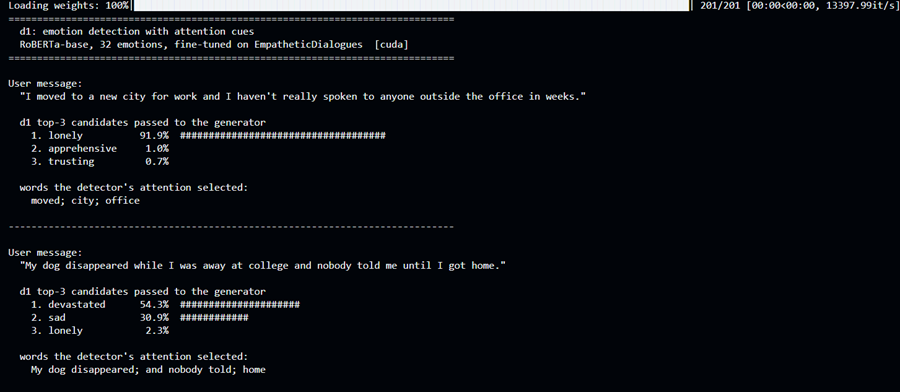
\includegraphics[width=0.95\linewidth]{figures/ch5_fig3.png}
\caption{The detector on two messages: three candidates, their confidence, and the words its attention selected}
\label{fig:5.3}
\end{figure}

\begin{figure}[htbp]
\centering
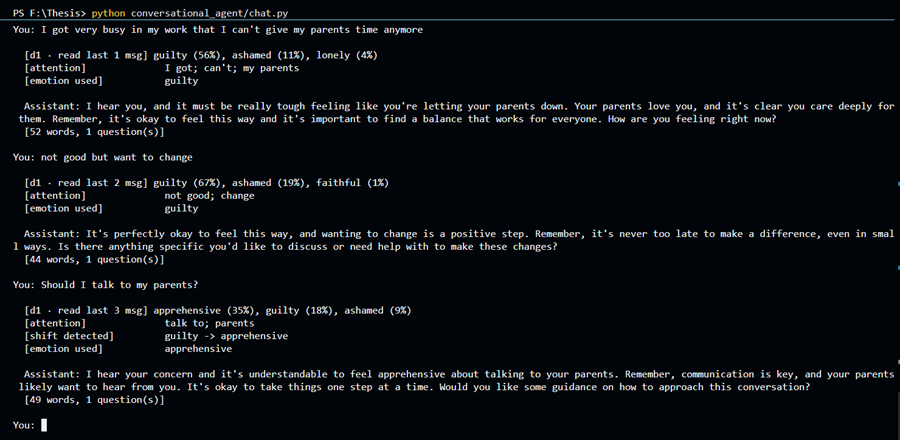
\includegraphics[width=0.95\linewidth]{figures/ch5_fig4.png}
\caption{Three turns of the agent, with the audit trail it prints before each reply}
\label{fig:5.4}
\end{figure}

\section{Analysis of Design Solutions}
\label{sec:5.2}

What each design accomplished was reported in section 5.1. It looks at one design question at a time to explain why they are different and then concludes by considering other design alternatives in comparison with criteria that are not measured by performance figures.

\subsection{Decoupled against Monolithic Designs}
\label{sec:5.2.1}

The main thesis question is: Is there a need for a separate model of emotion detection? There are four designs that do not include a detector that answer the same conversations and they fail in 3 different ways.

\textbf{A single model can only learn the style from the dataset it's trained on, not the desired behaviour:} the LoRA-tuned generator produces short and casual responses that rarely recognize the emotion, and it is last on empathy, emotion fidelity, and judges; it learned what it was trained to learn, the dataset itself does not have the desired behaviour. \textbf{With just zero emotion, the prompting leaves the model with nothing to work off of: }zero-shot prompting asks the one, required question in 22.7\% of the answers. Combining both tasks in one model narrows part of the gap, but \textbf{the one that is important to this paper:} the same-size single model achieves a high accuracy of 51.3\% on all rules, while remaining only marginally more faithful to the actual emotion than zero-shot prompting (24.7\% vs 25.7\%).

Since this comparison modifies the generator and also the design, we constructed the test which modifies only the design, the same of the final system, single-model prompt, no detector at all. It follows the rules more often than the decoupled system (73.7\% to 60.0\%), but its empathy and emotional fidelity are equal to the smaller single model (4.75, 27.0\%) and are raised to 5.05, 36.7\% when the detector and the per-emotion guidance are added to the latter. It is reported in full in Section 5.5.5 and is the best evidence in this thesis that has shown the second model to be worthy of its place.

\textbf{A larger single model is still better overall: }Qwen2.5-7B does better everywhere except structure (because it uses the same prompt as the same-size single model). Section 5.2.6 considers the trade-offs between the cost of decoupling and the possibilities it affords.

\subsection{Detector Alternatives}
\label{sec:5.2.2}

The detector was set to two findings. First, \textbf{it is more important what the detector is trained on than which network is used.} Retraining GPT-2 Medium on the situation descriptions from the dataset, but then using the user's unique message, gained approximately nine points of accuracy (56.9\% compared to 48.2\%); the largest single single detector accuracy improvement was retraining the detector on the actual text that GPT-2 was asked to produce.

Second, \textbf{for models of the same size, there are no significant differences on top-1 accuracy }(48.8-50.2\%) between encoders trained on the right input; only differences in quality of the ranking (85.0\% vs. 81.7-82.7\% top-5 for BERT and ELECTRA, respectively) can be seen (Figure~\ref{fig:5.5}, Tables 5.11 and 5.12). Two-stage design uses up ranking. ROBERTa-large increased the top-1 accuracy by 2.9 points at 7.4 times the training cost and did not change any measures of quality of replies in the pipeline (Section 5.4.3), and so RoBERTa-base was retained.

\begin{figure}[htbp]
\centering
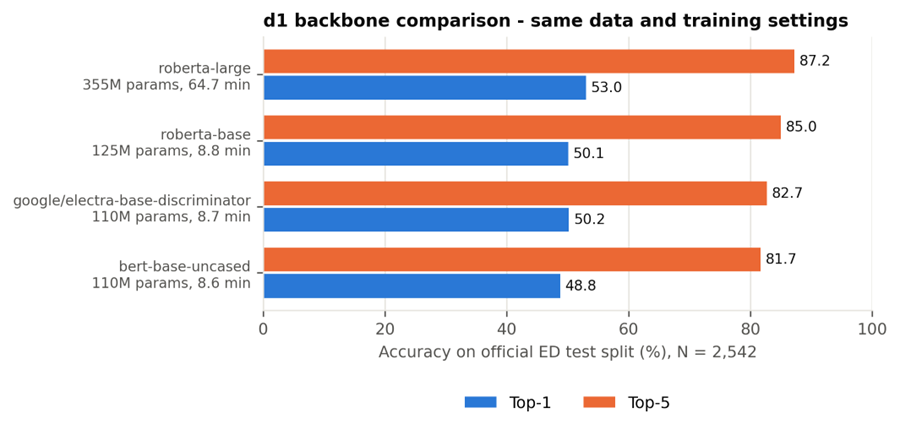
\includegraphics[width=0.95\linewidth]{figures/ch5_fig5.png}
\caption{Top-1 and top-5 accuracy of the detector candidates under identical training}
\label{fig:5.5}
\end{figure}

\subsection{Generator Alternatives}
\label{sec:5.2.3}

The generator determines how well the rules are adhered to, with Phi-4-mini at 65.3\% adherence, Qwen2.5-1.5B at 57.7\% and Gemma-3-4B at 22.0\%.

One might think that the most empathetic model of all is the instructive case, as it scores higher than Phi-4-mini on the empathy classifier and recognizes that 96.7\% of the time there is a feeling to recognize. However, it has an average of 133 words, 72\% of the responses exceed the limit and, in all the classifiers we measured, the system encourages longer responses (Section 5.4.4). Comparing similar length replies evens the playing field: in any band where both reply, Phi-4-mini holds up or just equals Gemma; and Gemma only outdoes Phi-4-mini at >120 words, where Phi-4-mini doesn't reply at all. Its apparent empathy is verbosity, and a system which is supposed to answer someone in distress, cannot disregard the length rule.

\subsection{Integration Alternatives}
\label{sec:5.2.4}

Making a connection between the two models is also a design decision - there are four different ways to do this and the difference lies in how much of the reasoning is asked of the generator. The two-stage design is able to enhance the emotion fidelity from 28.3\% to 36.7\% and the empathy from 4.89 to 5.05, which are reliable after correction, and shorten the replies from 80.4 words to 57.1 words, with the same detector and generator, and only the top-1 emotion and a general prompt. It requires 5.3 points in adherence to the rules which is an unreliable difference.

The benefit is dependent on the ability of the generator. The same change also affects Qwen2.5-1.5B, which drops adherence to 36.7\% and acknowledgement to 47.0\%, mirroring the results of the candidate-pick variant for this model (54.0\%): a small model provided with more room to reason becomes less compliant with the output format. The rules will not be dropped if a more detailed prompt is used; this can only be done with the bigger teaching-centered generator.

One drawback should be made explicit: this comparison involves the removal of three elements simultaneously: the top-3 selection, the emotion-specific guidance and the attention cues. The contributions of each of them were not distinguished, and it is listed as future work (Section 5.6.6) to separate them.

\subsection{Retrieval Augmentation}
\label{sec:5.2.5}

\textbf{How retrieval is used:} All the training conversations were inserted as a pair of messages with all-MiniLM-L6-v2 \cite{reimers2019sbert}. The detector's emotion was used to filter the pool of conversations to only those that contained the emotion at generation time, and the two most similar conversations (measured by cosine similarity) were retrieved and the human responses pasted on the system prompt as worked examples, above the same three rules \cite{lewis2020rag}. The second attempt further restricted the set to responses with a single question and explicitly reminded the person that the response must include one question mark.

\textbf{It reduced adherence to rules in both versions:} 54.3\% and 43.7\% compared to without retrieval (63.7\%). The explanation is in the data: only 4.3\% of the real listener replies adhere to all 3 rules, and what is retrieved is therefore a style that is contrary to the instructions provided in the same prompt. The percentage of compliance with the one-question rule was 76.0\% for the first version, and 57.0\% for the second version (after filtering examples and repeating the rule, the acknowledgement percentage dropped from 70.3\% to 57.0\%).

\textbf{Nothing was retrieved:} This is reported on all the same measures as all other systems because a design that sacrificed rule adherence may still be worth keeping if it gained in other aspects. It did not: empathy 4.85 compared to 4.80 without retrieval and emotion fidelity 27.7\% compared to 26.0\% both of which are very much smaller than the uncertainty on those estimates (Section 5.4.2) and the spread of its empathy scores is the widest of any system. It is the one design in Table~\ref{tab:5.1} that the model judges never scored. The three cells of the first attempt are not blank, but instead indicate that they cannot be recovered because their outputs were overwritten before the measures were computed. In this activity, participants can see examples of how people react in real life situations that go against explicit behavioural rules -- not reinforce them.

\begin{table}[htbp]
\centering
\scriptsize
\caption{Retrieval augmentation on every measure, against the same pipeline without it}
\label{tab:5.3}
\begin{tabularx}{\textwidth}{@{}lXXXXXX@{}}
\toprule
\textbf{Variant} & \textbf{Ack (\%)} & \textbf{One question (\%)} & \textbf{All rules (\%)} & \textbf{Mean words} & \textbf{WASSA empathy} & \textbf{Emotion validation (\%)} \\
\midrule
Without retrieval & 70.3 & 87.3 & 63.7 & 35.2 & 4.80 (SD 1.33) & 26.0 \\
With retrieval, attempt 1: 1-2 retrieved examples & not recoverable & 76.0 & 54.3 & not recoverable & not recoverable & not recoverable \\
With retrieval, attempt 2: filtered examples + rule reminder & 57.0 & 78.0 & 43.7 & 34.0 & 4.85 (SD 1.46) & 27.7 \\
\bottomrule
\end{tabularx}
\end{table}

\subsection{Assessment against Criteria beyond Performance}
\label{sec:5.2.6}

It's not just about performance and the other options differentiate clearly in that regard. These two designs, the fine-tuned baseline and the retrieval pipeline, are also the two that have the highest cost of change. All the single-model designs of any size have their emotional decision within, there is nothing to look at and nowhere to put a safeguard. The emotion is exposed in the decoupled designs, and the one picked is the most: three candidates, the picked one, the words that prompted it, the detector, the guidance and the generator are all separately replaceable.

The performance measures contradict each other and it is the two tables in Section 5.1 that resolve the issue of choice between the two. On what the replies do (Table~\ref{tab:5.1}) the final system is mid-table: it follows all three rules less often than the largest single model did or it was prompted to do, and it expresses the person's real emotion more often than any other system. In terms of how empathetic they are judged to be as it is second of eight, bettered only by the single model with 7.6 billion parameters, which requires 1.9 times its parameters and 62\% more GPU memory, and first among those that fit the requirement N1 in Section 3.1.2.

That's what the selected design is saying in so many words: at that scale, there's nothing more emotionally faithful than it, there's no system of that size that's rated more empathetic, and it's the only design here whose emotional decision can be read, logged or intercepted. What it loses is adherence to rules, and Section 5.5.5 quantifies just how much.

\section{Final Design Adjustments}
\label{sec:5.3}

Testing of the early pipeline, consisting of a GPT-2 Medium detector and a Qwen2.5-1.5B generator, revealed some flaws. Below are each of the adjustments that were made in response to a measured result, and each was re-evaluated on the same 300 conversations prior to being retained. 

\subsection{Adjustments to the Detector, the Generator and the Prompt}
\label{sec:5.3.1}

When the first detector was measured on the input that it receives, there was a mismatch between training and use: it was trained on situation descriptions of the dataset and in that case, the name of the feeling is nearly explicitly stated; in the case of the pipeline, it was given the user's conversational message. The detector was retrained on the first messages and, after the comparison of the encoders in Section 5.2.2, GPT-2 Medium was substituted by RoBERTa-base. Now it's accuracy is describing what it really does, and its ranking is good enough to be the top-3 selection.

Of the comparisons in Section 5.2, three were retained after being re-measured on the same conversations. \textbf{Replaced the generator:} Phi-4-mini obeyed the rules more frequently than Qwen2.5-1.5B, thus d2 was set to 4-bit version of Phi-4-mini.\textbf{ The emotion decision was made in its own call: }the correct emotion is in the top 3 of the detector in 76.5\% of the conversations, the top label is wrong in about half of the conversations, and an earlier version that decided and replied in a single call had harmed the rule-following. \textbf{There are 32 different emotions and guidance for each is fairly general:} "the user is feeling X". But what about a response to loneliness versus a response to pride? These combined, and with detector and generator fixed, yielded an increase in emotion fidelity from 28.3\% to 36.7\% and an increase in empathy from 4.89 to 5.05, both reliable after correction, with a 5.3-point drop in rule adherence not being reliable; replies also went down from 80.4 to 57.1 words, again within the limit.

The original design used an attention mechanism which was never implemented. However, a verification check revealed that the default implementation of attention in the library does not return any attention weights and does not throw any error, so the feature would have been silently inactive and seemed to be working. The adjustment includes an option to return weights, to stop if weights are not available, to merge adjacent fragments back into full words and to pass only the top 40\% of tokens (up to three phrases) so that the cues do not simply repeat the message.

\subsection{From Single Replies to a Conversation}
\label{sec:5.3.2}

This evaluation is based on 1 message and 1 response. A question that could not be assumed but had to be measured is how much of the conversation should the detector read if turned to the agent specified in Section 4.2.7?

\textbf{The reason why the dataset cannot answer it: }The maximum number of turns in EmpatheticDialogues conversations is 4, and the median is 2 turns, and the gold emotion does not change in the conversation, there is no multi-turn emotion shift in the data to tune a window against. Instead, we wrote conversations that include the kinds of changes that a real support conversation would generate, most notably the "I'm fine, actually I'm not" pattern, where the last message in the conversation communicates the opposite of how the person is really feeling. This is not statistical evidence, it is illustrative evidence for a design choice -- \textbf{this is our own opinion as to what a listener will hear in the column.}

\textbf{Across 10 short conversations,} with a deliberate change, moving from one turn to four shifted the prediction to what a listener in five of these would hear; in three the prediction was not changed; in two the prediction was changed -- one neighbour of the intended emotion was replaced by another -- but in none of the turns did a correct single-message reading become incorrect. The easiest example is the one that initiated this test - "I am okay. Well, not properly" is read as content at 72\% confidence, and "Someone yelled at me today very badly" with the previous turn as angry.

\textbf{However, a window can be too large:} Table~\ref{tab:5.4} opens up the window on four long conversations (6-8 turns), and four turns is the largest window that does not affect the quality of any of them. When six turns two of the four move away from the listener's reading, one of them, the break-up conversation, is correct at four turns (lonely, 61\%), but guilty at 64\% when the anger of the previous turns comes back into the window. With increased confidence, the control remains anxious at all widths, and the damage is not caused by the length of the input, but by stale emotions competing with the current one. We don't omit the burnout conversation, neither setting recovers it.

\textbf{The fixed 4-turn} window was kept as it gave the same answer as a 4-turn window that only widened when the detector was not sure, using the median of the detector confidence of 0.632 as the threshold in all 10 scenarios. The generator did not need this test as it is a large context window instruction following model, not a short text classifier.

\begin{table}[htbp]
\centering
\scriptsize
\caption{The same test on four long conversations, where a window can become too wide}
\label{tab:5.4}
\begin{tabularx}{\textwidth}{@{}lXXXXXXXX@{}}
\toprule
\textbf{Conversation} & \textbf{Turns} & \textbf{A listener would hear} & \textbf{Last 1} & \textbf{Last 2} & \textbf{Last 3} & \textbf{Last 4} & \textbf{Last 6} & \textbf{Last 8} \\
\midrule
work stress -> burnout -> quiet despair & 8 & devastated / empty - NOT ordinary work stress & content (50\%) & lonely (62\%) & ashamed (41\%) & lonely (20\%) & ashamed (49\%) & ashamed (54\%) \\
breakup -> anger -> loneliness & 7 & lonely / sad & anxious (31\%) & lonely (26\%) & lonely (40\%) & lonely (61\%) & guilty (64\%) & - \\
illness scare ending in relief & 7 & grateful / relieved & content (78\%) & content (36\%) & faithful (32\%) & hopeful (33\%) & faithful (25\%) & - \\
Control: emotion stays constant throughout & 6 & anxious (should stay stable at every window) & anxious (25\%) & anxious (30\%) & anxious (66\%) & anxious (75\%) & anxious (81\%) & - \\
\bottomrule
\end{tabularx}
\end{table}

A web demonstration of the agent was prepared for Hugging Face Spaces, with disclaimers and crisis resources shown on the page.

\subsection{Adjustments That Were Rejected or Deferred}
\label{sec:5.3.3}

Not all candidates' changes passed the evaluation. Retrieval augmentation reduced rule adherence from 63.7\% to 43.7\% and was rejected (Section 5.2.5), while a larger detector did not improve any of the measures of reply quality within the pipeline, although it was 2.9 points more accurate when used alone (Section 5.4.3).

There were two changes that were \textbf{postponed.} The boilerplate rate of 58.7\% would likely be decreased with the introduction of a repetition penalty, but generating the boilerplate replies would have negated the judge scores and human-evaluation items already created on those. The first item of future work (in Section 3.4) is a pre-generation crisis filter, which must be installed before any public deployment.

\textbf{Fine-tuned baseline:} a monolithic LoRA baseline had a configuration mistake, which has been corrected. Averaging 200.7 words and 7.07 questions per reply, 99\% of its answers were padded with the end-of-turn token (which meant they were limited to 250), and the collator removed padding from the loss, so it wasn't trained to stop: We retrained it using the padding token from the model, added start-up check to abort training if the end-of-turn padding would be masked, and chose the best epoch based on the validation loss. The corrected model concludes its response normally, as its responses do not exceed the word limit (10.0 words, wherein none exceeded the word limit), and adheres to rules in 22.3\% of cases. All results given in this thesis refer to the corrected baseline; the original run itself is given here only as an error documented.

\section{Statistical Analysis}
\label{sec:5.4}

Some of the differences so far reported are large enough to build on, others are not. This section is a divider between the two.

\subsection{How the Tests Were Done}
\label{sec:5.4.1}

All 300 conversations are answered by every system, and every detector is tested on all 2,542 conversations, making all comparisons paired, and allowing for comparison conversation by conversation, not just in aggregate. In the case of binary (yes/no) responses, e.g., whether a reply followed all the rules or expressed the true emotion, we employ McNemar's exact test which examines only the conversations in which the two systems disagree. For scores (e.g., empathy scores, judge ratings) we apply the Wilcoxon signed rank test that makes no assumption about the shape of the distribution. For each comparison there is also a 95\% bootstrap confidence interval based on 10000 resamples with seed 42, so that the size of a difference is not only apparent, but also visible.

The final system is compared with seven baselines on each measure, so p-values are adjusted within each measure by the Holm-Bonferroni procedure. \textbf{A difference is considered real if the adjusted p value is < 0.05 and the confidence interval does not contain zero.} Independent group comparisons (e.g., error-propagation analysis) are made using Fisher's exact test and the Mann-Whitney U test instead.

\subsection{The Final System against Each Baseline}
\label{sec:5.4.2}

Figure~\ref{fig:5.6} displays all comparisons together: the difference between the final system and each baseline on the three headline measures and its confidence interval, coloured by whether it survives correction. It is woven with three patterns.

\textbf{Empathy and emotion fidelity is reliably enhanced on each and every similar design.} The empathy score is higher than all baselines (except the largest single model) by 0.16 to 0.25 points, and\textbf{ by 0.30 points over the same generator alone }(95\% CI [+0.19, +0.41], adjusted p < 0.001). Emotion fidelity is also increased compared to all baselines except the largest single model (8.3 to 18.3 points, all adjusted p < 0.013). The improvements are not due to the size of the generator as the single-model baseline based on our own generator performs no better than the 1.5 billion parameter generator on these two measures (Section 5.5.5).

\textbf{We do not claim the difference between the rule adherence and the same-size single model after correction }(raw p-value of 0.032, Holm corrected p-value of 0.095). The final system is reliably better than zero-shot prompting, the fine-tuned model and the retrieval pipeline, no different from the initial pipeline or top-1 Phi-4-mini prompting, and reliably worse than its own generator used alone (-13.7, p = 0.002) and the largest single model (-22.3). It outperforms the same-size single question model by 19.0 points (p < 0.001) on the one-question rule alone.

\textbf{The one that has been corrected the most and is truly better on rules and empathy} is Qwen2.5-7B, which leads on overall rule adherence (+22.3 points), acknowledgement (+16.7), the one-question rule (+6.3) and empathy (+0.71). We report as it is.

\begin{figure}[htbp]
\centering
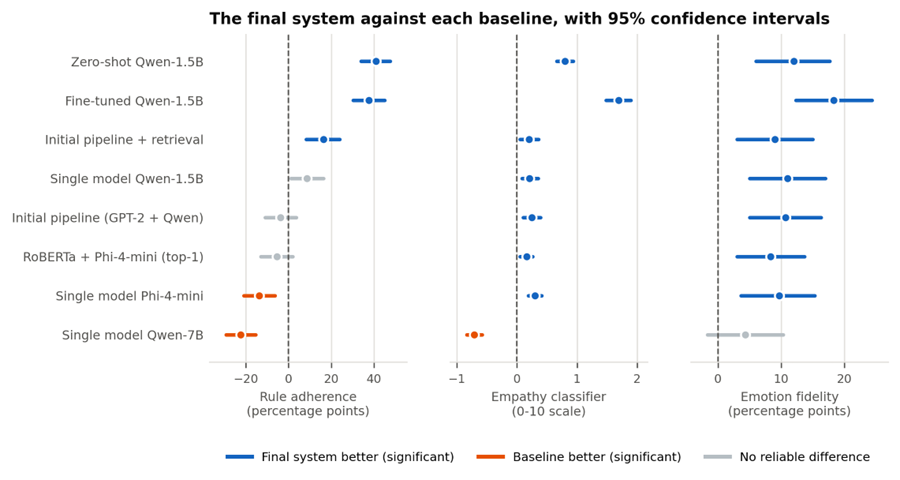
\includegraphics[width=0.95\linewidth]{figures/ch5_fig6.png}
\caption{The final system against each baseline on three measures, with 95\% confidence intervals}
\label{fig:5.6}
\end{figure}

\subsection{Is the Detector the Bottleneck?}
\label{sec:5.4.3}

The quality of the reply would be dependent on the accuracy of detection, and a better detector would result in better replies. Three tests declare it to be no.

\textbf{Replies based on a wrong label are no worse:} splitting each pipeline's replies by whether the detector matched the gold label shows no reliable loss of adherence of any pipeline: 61.2\% vs 66.0\% for the initial pipeline (p = 0.40) and no reliable difference for the final system (p = 0.096). Empathy is unaffected as well (4.83 against 4.78, p = 0.72).

\textbf{Replacing GPT-2 with the more accurate RoBERTa detector does not affect things downstream: }the emotion fidelity (p = 0.91) and adherence to rules (p = 0.09) do not change with the change of detector, but there is a significant difference between the two when they are used as classifiers.

\textbf{Similarly, doubling the detector did not make a difference:} When the detector was replaced with RoBERTa-large and the entire final system was rerun on the 300 conversations, the detector's accuracy improved by 3.0 points on the conversations, but nothing changed for adherence to the rules (p = 0.60), empathy (p = 0.85), emotion fidelity (p = 0.85), or the one-question rule (p = 0.60).

Here is one related result. The stage-1 choice is matched by the gold label in 42.3\% of the conversations, compared to the detector's 50.3\% (difference -8.0 points, CI [-13.3, -2.7] and p = 0.005), while the gold label is matched by the detector in 42.6\% (difference -7.7 points, CI [-12.9, -2.5] and p = 0.005). It is a real difference and the improvement of the two-stage design is not attributable to better emotion selection (Section 5.6.2).

All these together, detection accuracy is not what constrains reply quality, which is why it is worth spending the memory budget on the generator rather than the detector.

\subsection{What the Empathy Classifier Is Worth}
\label{sec:5.4.4}

The Spearman correlations range from 0.14 to 0.54, p < 0.02, with longer replies being more likely to be classified as empathy. Thus, a verbal system may appear empathetic, but not be, just as LLM judges have reported \cite{zheng2023judge}. This has an impact on two comparisons in opposite directions. It provides a complete explanation of the high score of Gemma-3-4B (Section 5.2.3). And it helps the final system's case over the top-1 prompting, because the final system gets the higher score with shorter replies (57.1 vs. 80.4 words). This also does not account for the largest single model, which has an average of 52.9 words for its replies.

Because of the dependence of a number of conclusions on the empathy classifier, we assessed its performance with the judges on the 512 replies scored. It correlates with the judges well (rho = 0.74) across systems, but it is in disagreement on one system: the single system developed on our generator is ranked 2nd by judge empathy and 7th by classifier score. Across individual responses, agreement is weak but genuine (rho=0.30, p<0.001) and does not disappear when length is controlled (partial rho=0.25), so it is not just a matter of a shared preference for long responses. The within-system agreement is weak (rho = 0.05 to 0.41, reliable in four of eight systems), compared to inter-judge agreement which is 0.69.

This is the proof on which we act throughout: the classifier compares averages of the system, never a single reply, and always against a second measure.

\subsection{What the Judges Separate, and How Much They Agree}
\label{sec:5.4.5}

Against the same-size single model the final system is rated reliably higher on empathy (+0.70, CI [+0.39, +1.01], p < 0.001), relevance (+0.44, p = 0.023) and overall (+0.44, p = 0.001), and reliably higher overall than the initial pipeline (+0.65), zero-shot prompting (+1.18) and the fine-tuned model (+2.73), all p < 0.001. Compared to the largest single model it is lower on empathy (-0.30) and overall (-0.21); however, neither of these differences is significant after correction (p = 0.073 and p = 0.109). \textbf{The judges do not differentiate between the three systems using the same generator at all: }top-1 prompting (overall +0.04, p = 0.71) and that generator alone (overall -0.10, p = 0.16).

The two judges' own correlation is rho = 0.69 for empathy and 0.68 overall, and their rankings of the eight systems are identical except for one pair that differ by 0.03. The literature suggests that they should be drawn from different model families to avoid bias from a single model \cite{verga2024}, which is what we have done.

\subsection{Human-Evaluation Statistics}
\label{sec:5.4.6}

All forty participants completed the study and none were excluded as they all consented. Each participant rated all three systems in all eight situations; thus, differences in rating systems cannot per se create an effect because a person who rates all three systems as such is doing so. The tests are therefore Wilcoxon signed-rank tests on per-participant mean ratings, with the Holm correction across the nine tests (three system pairs and three scales), and 10,000-sample bootstrap confidence intervals with the same seed as used elsewhere. Each of the six comparisons made with the final system is significant after correction, and none of the confidence intervals contain zero. Against the same-size single model it gains 0.64 points on empathy (95\% CI +0.41 to +0.88, adjusted p = 0.0001), 0.60 on contextual relevance (+0.33 to +0.88, adjusted p = 0.0017) and 0.65 on supportiveness (+0.41 to +0.89, adjusted p = 0.0002). Against the larger single model it gains 0.46 on empathy (+0.25 to +0.69, adjusted p = 0.0015), 0.47 on relevance (+0.25 to +0.71, adjusted p = 0.0039) and 0.50 on supportiveness (+0.29 to +0.72, adjusted p = 0.0008). After correction, the two single models cannot be distinguished from each other on any scale, and the additional parameters of the larger model do not provide any measurable improvement in the people's rating of its replies.

The final system was selected 196 times out of 320 on the preference question, 61.3\% (95\% interval 55.7\% to 66.6\%) which a 2 sided binomial test shows is far from the chance rate of a third (p<0.001). The larger single model was selected 21.6\% of the time and the same size model 17.2\% of the time, both also significantly different from chance, but in the opposite direction. The result is not dependent on a few situations or a few persons: the final system was preferred in all eight situations by 18 to 29 of the 40 persons and 22 of the 40 persons gave it their own highest average rating, as compared to 9 persons each of the two baselines. There is little consensus among participants and this is not set aside. Intraclass correlation for the 1-5 ratings is 0.084 for empathy; 0.075 for relevance; and 0.082 for supportiveness; and Fleiss' kappa for the preference question is 0.018. When correctly interpreted, these say that the rating that any one person gives to any one person contains little information, but that the preference is a consistent mild majority in every situation, and not a strong consensus in any situation; there is no situation in which most of the raters agree on the same reply for the same reason. What the study demonstrates is the sum total, and the sum total is in the same direction for all eight situations, on all three scales and the paired tests. Human ratings and the model judges agree where they overlap. The two are also correlated at a Spearman's rho of 0.516 (p = 0.049) and a Pearson's r of 0.537 (p = 0.039) over the 15 system-situation pairs that the judges also rated, and both rank the three systems in the same order: the final system first, the larger single model second, and the same-size model third. The judges give the end result of the final system 8.7 and the bigger single model 8.6 in those five cases. This is why the overall preference of the panel for the larger model, as reported in Section 5.1.5, is obtained. The wider judged set and not from the situations people saw.

\subsection{Limits of the Analysis}
\label{sec:5.4.7}

All of the above are subject to three limits. The 300-conversation sample will have a greater ability to detect a few percentage-point differences but less ability to detect smaller differences, and the 64-conversation judge sample has even less ability to detect differences. Emotion fidelity is based on our own detector reading text it has never seen. Within each measure, and only within each measure, Holm correction was applied, and the seven baselines were treated as one family of comparisons; that is a choice, and we state it rather than leave it implicit.

\section{Comparisons and Relationships}
\label{sec:5.5}

In this section, the results are compared with published work, where it is appropriate, and the relationships between variables uncovered by the experiments are reported.

\subsection{Compared with Published Work}
\label{sec:5.5.1}

The results of our detector are compared with the published results in Table~\ref{tab:5.5} on the same 32 emotions. When reading it, two things must be kept in mind: what the system reads, which may be a whole conversation, the situation description or only the speaker's first message; and which partition the number is from.

Our detector's 50.3\% exceeds every joint recognition: and-generation model listed, at 30.6-41.2\% \cite{lin2019moel,majumder2020mime,sabour2022cem,zhou2023case}, and the personality-aware models at 45.4-48.3\% \cite{wu2025traits}. There are four reasons for that and only the last is a choice we can take pride in.

\textbf{1. Our detector is initialised from a much stronger encoder:} pre-trained on approximately 160 GB of text, whereas MoEL, MIME, CEM and CASE initialise their word representations from GloVe vectors and train their encoders only on EmpatheticDialogues. The only joint model in the table, which is built on pre-trained components, is RoBERTa-GPT2, which is the only one that matches us.

\textbf{2. It does one thing:} Our joint model is trained and selected on emotion recognition as an auxiliary task and shares its capacity with response generation, while the joint models learn emotion recognition as an auxiliary task only.

\textbf{3. It is selected based on the measure it is being used for: }The checkpoint saved is the one with the best validation accuracy and the candidate selected is the one with the best top-5 accuracy, since the design uses a ranking, not a single label.

\textbf{4. It is trained on the text it will actually be given: }Training on the situation description, as the first version of this project did, reads as a better number and is a worse detector: the same model loses about nine points when moved to the message a user really writes (Section 5.3.1).

The fair summary is that it achieves this accuracy when it reads less, one message, not a full conversation, as would a live system.

\begin{table}[htbp]
\centering
\scriptsize
\caption{Emotion recognition on EmpatheticDialogues in published work and in this thesis}
\label{tab:5.5}
\begin{tabularx}{\textwidth}{@{}lXXXX@{}}
\toprule
\textbf{System} & \textbf{Input and split} & \textbf{Top-1 (\%)} & \textbf{Top-5 (\%)} & \textbf{Source} \\
\midrule
EmpDG (Li et al., 2020) & Joint model, full conversation & 30.64 &  & Qian et al. 2023, Table 1 \\
MoEL (Lin et al., 2019) & Joint model, full conversation & 30.75 &  & Qian et al. 2023, Table 1 \\
MIME (Majumder et al., 2020) & Joint model, full conversation & 31.21 &  & Qian et al. 2023, Table 1 \\
KEMP (Li et al., 2022) & Joint model, full conversation & 36.57 &  & Qian et al. 2023, Table 1 \\
CEM (Sabour et al., 2022) & Joint model, full conversation & 37.81 &  & Qian et al. 2023, Table 1 \\
CASE (Zhou et al., 2023) & Joint model, full conversation & 38.92 &  & Qian et al. 2023, Table 1 \\
ESCM (Yang et al., 2023) & Joint model, full conversation & 41.19 &  & Findings of EMNLP 2023 \\
Personality-aware model (Wu et al., 2025) & Joint model, text-only ED & 45.4 &  & COLING 2025 main.598, Table 4 \\
EmpSOA & Joint model, text-only ED & 48.3 &  & COLING 2025 main.598, Table 4 \\
fastText (Rashkin et al., 2019) & Classifier, situation description & 43.0 &  & ED paper \\
DeepMoji (Rashkin et al., 2019) & Classifier, situation description & 48.0 &  & ED paper \\
OURS - RoBERTa-base d1 & Classifier, first utterance, TEST split & 50.3 & 84.3 & this work \\
\bottomrule
\end{tabularx}
\end{table}

By contrast, published generation scores cannot be compared with ours: their test set is much bigger, and the scores drop as the test set increases, from 32.3\% at 50 replies in their test set to 15.6\% at 300; whereas published BERTScore values refer to a reply that is compared with a reference answer that comes after a multi-turn context. Thus, we report measures that are not found in published work, such as rule adherence, an independent empathy classifier, emotion fidelity and paired significance tests.

Human evaluation enables comparison of direction, if not of size: people in published studies strongly prefer LLM replies to those of purpose-built empathetic models, rating ChatGPT at 4.64 out of 5 compared to 3.08 for CEM \cite{qian2023llm}.Our own study confirms this and takes one step further: the 40 participants preferred the final system in 61.3\% of the choices, a single model almost twice the size in 21.6\% of the choices, and a single model of its own class in 17.2\% of the choices, and rated it higher on all three scales. We have seen that a small general model with a separate emotion detector is preferred to a larger general model without an emotion detector, whereas published work shows that a large general model is preferred to a small purpose-built model. The protocols vary, so 5-point ratings, A/B preferences and our 3-way choice are only comparable in terms of direction.

\subsection{What Detector Accuracy and Generator Capacity Each Buy}
\label{sec:5.5.2}

In all three tests of Section 5.4.3, the user never received a gain of more than 2 to 3 points in the detection accuracy. The key is in the shape of the errors: an answer for\textit{ terrified} when the person was \textit{afraid }is still an answer for fear, and the same nearness is what makes the top-3 candidate set worth passing on, as opposed to the single most probable, which was correct only 50.3\% of the time. The emotion fidelity increase was more important than the accuracy of the finding: per-emotion two-stage prompting increased the emotion fidelity by 8.3 points, which is more than any detector upgrade we tested, with detector and generator unchanged.

Only a generator capable of following the richer prompts will be helped by the richer prompts. The same additions that leave Phi-4-mini's rule adherence unchanged while raising its empathy and emotion fidelity lower Qwen2.5-1.5B's adherence from 57.7\% to 36.7\% (Section 5.2.4), the earlier candidate-pick variant showed the same pattern on the smaller model, and adherence under a plain single-model prompt climbs from 51.3\% at 1.5 billion parameters to 82.3\% at 7.6 billion. The implication is that the complexity of instruction should be aligned with the capacity of the generator, and that in the case of less than a few billion parameters, it is better to choose a simpler prompt.

\subsection{Cost: Parameters, Memory and Time}
\label{sec:5.5.3}

Parameters by themselves don't determine the cost of running a system, as the system loads two models and calls the generator twice in every reply. Hence, we have measured the peak GPU memory and response time for the final system and both single models on the same 50 conversations, on the RTX 4060 used throughout. The measurements are provided in Tables 5.30-5.33, and are compared to the other systems in Table~\ref{tab:5.6}.

The final system achieves \textbf{97.5\%} \textbf{of the overall judge score} at 52.0\% of the parameters of the Qwen2.5-7B single model, maintains 87.7\% of the empathy-classifier score and 72.9\% of the rule adherence, and surpasses it on emotion fidelity. It does this with \textbf{38\% less peak GPU memory,} and no statistically significant difference in response time (CI [-0.03, +0.56] s, p = 0.10); per generated token the two are virtually indistinguishable (65.7 ms vs. 65.4 ms; p = 0.91). The additional operations of the decoupled design are inexpensive: detection + cue extraction = 0.016 s, and the stage-1 call = 0.29 s, or approximately 7\% of the time per reply.

These are two honest qualifications. The Qwen2.5-1.5B single model is lighter (2.90 GB) and 2.6 times faster, so the final system is efficient relative to the large model whose quality it approaches, not relative to the smallest baseline, whose replies are reliably less empathetic. The measurements are for one GPU and 50 messages and therefore indicative only.

\subsection{Do the Response Rules Measure Something That Matters?}
\label{sec:5.5.4}

One of our headline measures is adherence to rules, and the rules themselves must be justified: It's only a virtue to adhere to the rules if the rules are for something worth doing. The origin of each rule, and the measured effect, which is calculated within each system by subtracting the mean of that system and the effects cannot be due to differences between systems.

\textbf{Acknowledging the feeling} is the \textit{emotional reactions} mechanism of EPITOME is a framework of empathy in text-based support that is based on existing empathy scales \cite{sharma2020epitome} and the mechanism of emotional reactions is the acknowledgement of the feeling. Within the same system, in our data, replies that acknowledge score 0.36 points higher on the empathy classifier (p < 0.001, 3,300 replies); the judges point the same way but not reliably.

\textbf{A single question is a balance between two things: }a reply with no question, and several questions, which counselling guidance warns against \cite{samhsa2019tip35} and which only 4.7\% of the listener replies in the dataset do. \textbf{There is no automatic reward for this rule,} so we offer it as a usability and safety requirement, which can be seen in the failure mode of the fine-tuned baseline, and not as a way to a higher score.

\textbf{Keep a reply to within 120 words} so it is easy for someone in distress to read. The two measures disagree here: the judges rate the replies in the same system 0.65 points higher on empathy (p = 0.006), while the classifier rates them 0.22 points lower, the known length preference of the classifier. We follow the judges, since they read the text, not a proxy that is sensitive to length.

To summarise, two of the three rules are supported by published practice and our own data, and the third is supported by practice but not our automatic measures. The only test to settle it is the human study, which is ongoing.

\subsection{What the Detector Itself Contributes}
\label{sec:5.5.5}

All comparisons so far have been with a fixed generator, but with varying conversations and decoding. The test that isolates the design provides the final system's own generator with the single-model prompt and no detector whatsoever. The result is illustrated measure by measure in Figure~\ref{fig:5.7}, as the single model writes 29\% longer replies.

\textbf{The gains belong to the design, not to the generator: }Switching from Qwen2.5-1.5B to Phi-4-mini as a single model increases rule adherence significantly (51.3\% to 73.7\%, p < 0.001), but does not increase empathy (4.84 to 4.75, p = 0.18) or emotional fidelity (25.7\% to 27.0\%, p = 0.70), so a larger generator alone does not purchase the empathy we report. The three candidates and the per-emotion guidance, when added to the same generator, result in an increase of empathy to 5.05 (p < 0.001) and emotion fidelity to 36.7\% (p = 0.007). The empathy gain is the more robust of the two: it persists with shorter replies and increases with length control; the fidelity gain, by contrast, decreases with length control (p = 0.13).

\textbf{The price is adherence to the rules,} the decoupled system adheres to all three rules less frequently (60.0\% vs. 73.7\%, p = 0.002), mostly by acknowledging it, and the one-question rule is not different, while every reply is within the length limit, with the generator fixed. The reason is that the rules are included in the prompt, and the per-emotion guidance and cue words are included in the prompt, too, but the single-model prompt includes only the rules. When length is kept constant, the acknowledgement difference is gone (p = 0.36) and the rule difference is just on the edge of significance (p = 0.04), meaning that part of the cost is length and part is real. The judges' scores are virtually indistinguishable (8.68 versus 8.78, p = 0.16), and are virtually the same at matched length.

The trade-off is that at an equal generator, the decoupled design will be more expressive of the person's emotion, will be more successful on an independent empathy classifier, will repeat itself less and write shorter replies, and will allow for logging, auditing or intercepting of the emotional decision, while paying for that with some adherence to the rules. It's an exchange, not a clean win and we're reporting it as such.

\begin{figure}[htbp]
\centering
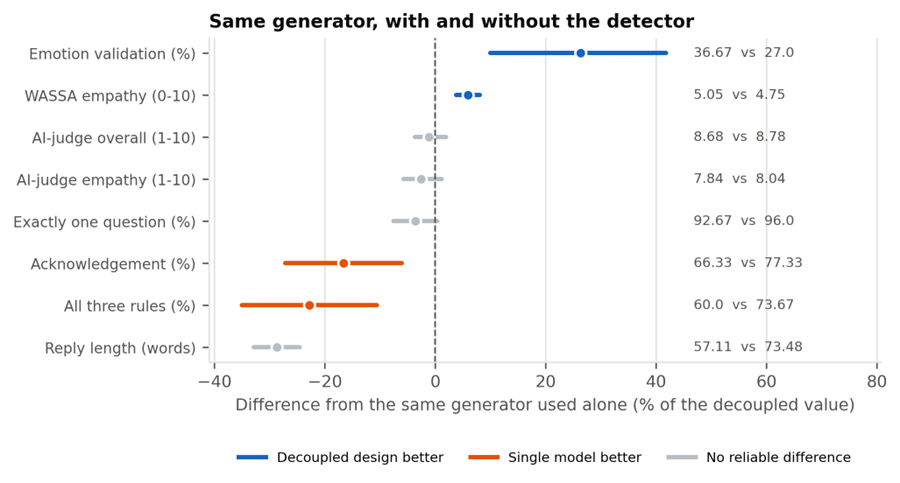
\includegraphics[width=0.95\linewidth]{figures/ch5_fig7.png}
\caption{The decoupled design against the same generator used alone, measure by measure}
\label{fig:5.7}
\end{figure}

\section{Discussion}
\label{sec:5.6}

This section reads the results as a whole -- what they said about the research question, why the surprising results came out that way, what the research cannot claim and what should come next.

\subsection{Answer to the Research Question}
\label{sec:5.6.1}

The question of the thesis was whether emotion detection and response generation can be separated to get better empathetic responses than a single model for both being asked on a single consumer GPU. The answer is a qualified yes, and the entire answer is in Table~\ref{tab:5.6}: our system, the same generator alone (which disconnects the design), and the larger single generator (the strongest that fits the hardware).

There are three true and one false statements in that table, read down the table. \textbf{It is parameter efficient}, being 52\% of the size of the larger model, and ranking second on the empathy panel of eight systems. \textbf{It is resource-efficient:} It's efficient with its 3.40 GB of GPU memory compared to 5.47 GB, and there's no consistent difference in its response time. \textbf{It is more emotionally faithful than either:} 36.7\% of its replies express the person's true feeling compared to 32.3\% and 27.0\%, and it repeats itself less than the same generator alone, while writing 22\% fewer words. What it doesn't score well at is rule adherence: 60.0\% to 73.7\% and 82.3\% and we don't say otherwise. Two cells are blank because we did not measure the single Phi-4-mini baseline, and do not attempt to estimate it.

\begin{table}[htbp]
\centering
\footnotesize
\caption{The three systems a reader has to choose between, measure by measure}
\label{tab:5.6}
\begin{tabularx}{\textwidth}{@{}lXXX@{}}
\toprule
\textbf{What a reader wants to know} & \textbf{Our system} & \textbf{The same generator alone} & \textbf{The bigger single model} \\
\midrule
What is it? & A detector and a generator, two short calls per reply & One model, one call per reply & One model, one call per reply \\
Models it loads & RoBERTa-base + Phi-4-mini (4-bit) & Phi-4-mini (4-bit) & Qwen2.5-7B (4-bit) \\
Total parameters & 3.96 billion & 3.84 billion & 7.62 billion \\
Peak GPU memory & 3.40 GB & not measured & 5.47 GB \\
Seconds per reply & 4.17 s & not measured & 3.91 s \\
Follows all three rules & 60.0\% & 73.7\% & 82.3\% \\
Empathy classifier (0-10) & 5.05 & 4.75 & 5.76 \\
Reply expresses the true feeling & 36.7\% & 27.0\% & 32.3\% \\
Empathy panel (three raters, combined) & +0.59 (2 of 8) & +0.53 (3 of 8) & +1.11 (1 of 8) \\
Replies using a stock phrase & 58.7\% & 72.3\% & 58.7\% \\
Words per reply & 57 & 73 & 53 \\
Shows which emotion it answered & Yes: three candidates, the chosen one, and the cue words & No & No \\
A safeguard can run before the reply is written & Yes & No & No \\
\bottomrule
\end{tabularx}
\end{table}

The empathy and fidelity gains are not due to the size of the generator, but to the structure, which is what the middle column represents: the same generator alone scores 4.75 and 27.0\%, and it does not gain anything on either measure when compared to the single model with 1.5 billion parameters (Section 5.5.5). The larger single model still outperforms on rules and on the empathy classifier, but the judges don't distinguish its empathy or its overall score from ours post-correction. So the argument for decoupling is not that separation is better than scale. It is about that separation, writing down an emotional decision that fits the hardware most people have.

\subsection{Why the Two-Stage Design Works}
\label{sec:5.6.2}

The most surprising result in the chapter is that the stage-1 choice is even less like the label in the dataset than the detector's own top choice (42.3\% vs 50.3\%), yet the system based on the stage-1 choice has the highest emotion fidelity and the highest empathy scores of any comparable system. This is reconciled by three observations.

First, EmpatheticDialogues assigns each conversation exactly one fine-grained label, which the speaker selects prior to writing anything; many messages seem to express a neighbouring feeling; since almost all disagreements are between neighbours, a choice that differs from the selected one label is often still a fair reading of the text. Second, replies based on a mislabeled label are as good as replies based on a correct one (Section 5.4.3): it is not the gold label per se that a reply requires, but the feeling of closeness to answer. Third, the improvement is apparent when per-emotion guidance is added. When you tell the generator how to answer loneliness, you change the answer from lonely to something else.

Since the selection and the guidance and cue words together were removed in our comparison, the percentages of the individual components are not distinguishable, but the accuracy result above indicates that the guidance is the most important component. This is also a smaller effect than the design's edge over single models, as there is little difference in the judges' assessment of the two-stage and top-1 variants, and the edge is seen in the finer measures of empathy and emotional fidelity.

\subsection{Objections, and When a Single Model Is the Better Choice}
\label{sec:5.6.3}

There are two objections which may be raised in this design and which were tested but not argued. 

\textbf{That a second model was not needed: }a model of the same size, and our own generator trained similarly, was equally unempathetic and unwarm in its responses; the detector was 125 million parameters, and a larger model would not affect the conclusion. Because real listener responses rarely adhere to the rules. 

\textbf{Retrieval would do the job more simply:} to manifest the generator the same emotion \cite{lewis2020rag} cut rule adherence in both the versions we built. We haven't developed the entire agentic system that was proposed to us, this evidence is about retrieval-augmented prompting, not agentic designs in general.

There's a case against our design, too. Given the sole objective of the best reply, our results on hardware which can store a 7-billion-parameter model are in favor of the larger single model. Decoupling should be used when the emotional reasoning must be evident: To audit the reason why a reply was written in a given way, to indicate to a user or a clinician what emotion was read, before any text is generated, or when components need to be replaceable individually. The two are not mutually exclusive, but the next most obvious experiment is to combine the detector and per-emotion prompting with a larger generator.

\subsection{Limitations}
\label{sec:5.6.5}

This work is constrained by seven limitations.

\textbf{Data:} EmpatheticDialogues is English, crowd-sourced and single-labelled, meaning that detection accuracy and suitability of the replies may not be held to transfer to the Bangla speakers and to those in real distress.

\textbf{Safety:} Suicidal ideation is not a label set, and there is no crisis safeguard other than interface disclaimers.

\textbf{Measures:} All automatic measures are proxies, the acknowledgement check is keyword based, the one-question rule is not rewarded by either empathy measure, the classifier has been trained on another domain and the length dimension, the judge panel currently consists of 2 members and the emotion fidelity is based on our own emotion detector.

\textbf{Number of conversations for generation:} 300; for judges: 64; and human study: 40 participants over 8 situations..

\textbf{Single turns:} The quantitative results are all basically for single turns, and the multi-turn agent was only evaluated on scenarios.

\textbf{Repetition:} 58.7\% of responses are repetitions of stock phrases.

\textbf{Efficiency:} Memory and time were measured for one GPU for 50 messages.

\subsection{Future Work}
\label{sec:5.6.6}

\textbf{Immediate Priorities}

\textbf{Incorporate a pre-generation crisis filter:} The filter is a ``must'' before public deployment and has reviewed safe responses \cite{who2023suicide}.

\textbf{Perform a component-wise ablation:} Perform an Ablation Study which unconfounds emotion selection, per-emotion guidance, and attention cues.

\textbf{Use a larger model generator:} Use the detector and per-emotion prompting with a larger generator model.

\textbf{Guidance written with practitioners:} three universal rules from published sources (Sharma et al; SAMHSA), and per-emotion guidance was not from published sources.The one part without any clinician is written by the authors external grounding. It needs to be created with practising Counsellors and Clinical. By interviewing them about their reactions to each type of situation, psychologists are able to assess a person's response style.requesting them to rewrite the 32 sets of instructions, and noting when their practice disagrees with ours, such an interview is not about any patient's, it is about professional practice, records. Already, these systems have been evaluated in published works based on counselling criteria.against clinicians themselves [Loh \& Raamkumar; Sorin et al.], and the standard is presentour guidance has not been kept to. The change is cost-effective as the guidance is Generation-time read is not followed by rewrite, which is no-training.

\textbf{Beyond English (Language Extension)}

\textbf{Compile localized data:} Obtain or create emotion-sensitive Bangla labelled conversations, including the naturally occurring code-mixed Bangla-English that people type.

\textbf{Retrain the detector:} trained from multilingual encoder with 125M Parameters, which is still still very low cost from a computational perspective.

\textbf{Rewrite per-emotion guidance:}Develop own guidance with native speakers, not translating guidance from English, and ensuring cultural correctness about the way in which emotions are addressed (e.g., loneliness, shame). (The separated architecture will enable it to retain the same generator while just changing the detector and guidance).

\textbf{Subsequent Steps}

\textbf{Control repetition:} Control text repetition in particular during the decoding time.

\textbf{Evaluate on real data:} Evaluate the system for actual multi-turn conversations and collect assessments from mental health professionals.

\textbf{Measure hardware performance:} Benchmark memory usage and response times for alternative hardware, such as CPU-only and mobile devices.
